\chapter{Requirement Specifications} \label{chap:reqs}

%\version{v1.10.2015}

\section{Existing System}
Currently, there is no online system which is being used by the Islamabad Pet & AVIAN Hospital G-10/4. Currently they are using manual system. No website and android application is still being used by the hospital.
\section{Proposed System}
Layman who buys the pet does not know the proper diet plans, their common diseases, treatment suggestions and sometime forget to fed . Pet Diet and Health care planner is an industrial project and it is designed and developed for the Islamabad Pets & AVIAN Hospital. It is a complete platform. The android application will support the user in generating pet diet plans, notify the owner on the proper timings that when your pet need food and also provide the pet disease and treatment suggestions. Users can take the appointment through android application and as well as through website. Website user can view information like hospital services etc as per as hospital requirement.

\section{Requirement Specification}
Requirements specification includes functional and as well as non functional requirements.
\subsection{Functional Requirements}
\begin{enumerate}[label=\alph*]
\item. Functional Requirement 1 (Registration)
Description:
Registration is compulsory for everyone who is using the Android Application for the first time. Registration will be perform to ensure the user account.
\item. Functional Requirement 2 (Login)
Description:
After the successful registration user is able to log in into the Android Application through the already registered email and password.
\item. Functional Requirement 3 (Add / View Pet Profile Details)
Description:
Android Application user can add and view the pet profiles. 
\item. Functional Requirement 3 (View/ Download Details)
Description:
Android Application user can view and download the diet plans and diseases details and treatment details. 
\item. Functional Requirement 3 (Generate Notification)
Description:
Application user can generate the alarm notification so that pet feed on proper timing.	
\item. Functional Requirement 3 (Take an Appointment)
Description:
Users can take the appointment through Android Application and as well as through website.
\item. Functional Requirement 5 (Website Application)
Description: 
Website user can take an appointment and view information like hospital services etc as per as hospital requirements.
\item. Functional Requirement 6 (Add as a Doctor)
Description: 
Android admin able to register doctor if assigned hospital id matches with the entered id.
\item. Functional Requirement 7(Logout)
Description:
Application users can logout at any time.
\end{enumerate}

\subsection{ Subsystem Functional Requirement}
\begin{enumerate}[label=\alph*]
\item. Login Processing
Description
Login activity is being performed on the system.
\item. Validation Check
Description
While log in into the system; system will perform validation either the email or password is correct or not.
\end{enumerate}

\subsection{Non Functional Requirement}
\begin{enumerate}[label=\alph*]
\item.	Performance
Least specification constraint is performed by the personal computer and which is necessary for every platform like android or web application. Memory, processor and operation system should match with the application.
\item.	Accuracy
If the application display the correct results like application is fetching correctly the pet diseases or treatment details etc according to user choice,  at run time then the application will be accurate.
\item.	Maintainability
The developer will perform the maintenance of both applications; android as well as web application if some issue occur.
\item.	Portability
It is true that now a day’s users demand the portable applications. Pet Diet and Healthcare is portable because it is available on both platforms android and as well as web.
\item.	Availability	
Application user is capable to perform and view application details on any time.
\item.	Flexibility
Pet diet and Healthcare planner is fully compatible and flexible system and easy to use for the end users.
\item.	Usability
The interface and Graphical User Interface design of the application is user friendly with no training required.
\end{enumerate}
\newpage
\section{Use Cases}
Uses case diagrams are very important because they help in understanding the whole system in a shorter time or quickly. Use case diagrams are designed for the both platforms android as well as for the web site.
\section{Use Case (System Diagram)}
Website user can view the information and make an appointment through website. 
Android Application user or pet owner can register then login into the system. After logging into the system the user can generate pet diet plan, view diseases details, add/view pet profiles, Add/view/delete food timings notification alarm, take/cancel appointment and log out.

\begin{figure}[H]
    \centering
    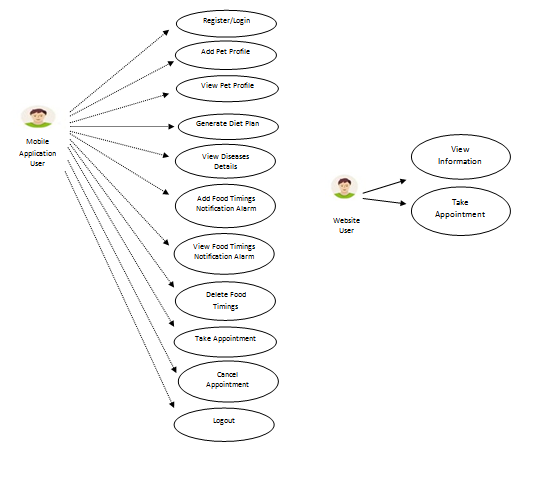
\includegraphics[scale=0.7]{301}
		\caption{Use Case (System Diagram)}
\end{figure}

\newpage
\subsection{Use Case (Website User)}
\begin{figure}[H]
  \centering
    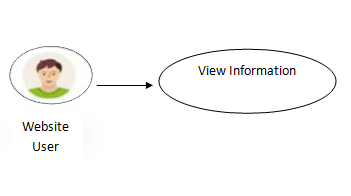
\includegraphics{42UseCase}
		\caption{View Information}
\end{figure}
Website user can view the every information which is provided by the pet hospital like services etc.
\begin{table}[ht]
\centering

\label{View Information (website)}
\begin{tabular}{|l|l|}
\hline
Name                     & View Information(website)                                                                                                                                        \\ \hline
Actor                    & Website user                                                                                                                                                     \\ \hline
Brief Description        & \begin{tabular}[c]{@{}l@{}}Website user is able to view the every information which\\  is mentioned on the website.\end{tabular}                                 \\ \hline
Flow of Events           & \begin{tabular}[c]{@{}l@{}}User can view hospital services, about us and doctors \\ detail etc or any further information provided by the hospital.\end{tabular} \\ \hline
Alternate Flow of Events & User will take an appointment.                                                                                                                                   \\ \hline
Pre-condition            & \begin{tabular}[c]{@{}l@{}}Should click on any button in the menu bar or scroll down\\ the cursor.\end{tabular}                                                  \\ \hline
Post condition           & User might take a decision of appointment.                                                                                                                       \\ \hline
\end{tabular}
\caption{View Information (website)}
\end{table}


\newpage
\begin{figure}[H]
  \centering
    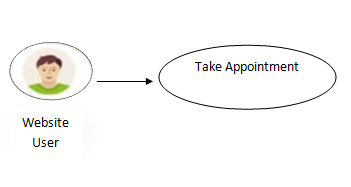
\includegraphics{43UseCase}
     \caption{Appointment (website)}
\end{figure}
By using the website feature our users will be able to take appointments online.
\begin{table}[ht]
\centering
\label{Appointment (website)}
\begin{tabular}{|l|l|}
\hline
Name                      & Appointment(website)                                                                                                                                                            \\ \hline
Actor                     & Website user                                                                                                                                                                    \\ \hline
Brief Description         & Website user is able to take an appointment.                                                                                                                                    \\ \hline
Flow of Events            & \begin{tabular}[c]{@{}l@{}}User will fill all the inputs text fields required for taking an\\ appointment. Like enter mobile number, pet name, date and times etc.\end{tabular} \\ \hline
Alternate Flow of  Events & User will view the information.                                                                                                                                                 \\ \hline
Pre-condition             & Fill all the input text fields.                                                                                                                                                 \\ \hline
Post condition            & Response email will be send to the user.                                                                                                                                        \\ \hline
\end{tabular}
\caption{Appointment (website)}
\end{table}




\newpage
\subsection{Use Case (Android User)}
\begin{figure}[H]
    \centering
    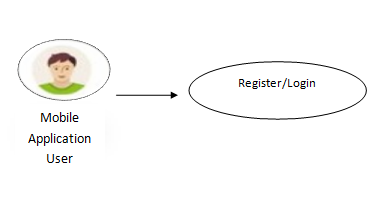
\includegraphics{31UseCase}
		\caption{Registrations/ Login}
\end{figure}
First of all Android Application User will register himself by filling registration form in order to login into the system or perform other activities.
\begin{table}[ht]
\centering

\label{Registrations/ Login}
\begin{tabular}{|l|l|}
\hline
Name                      & Registration/ Login                                                                                                                                                                                                                                                                   \\ \hline
Actor                     & Android Application User                                                                                                                                                                                                                                                              \\ \hline
Brief Description         & Registration is compulsory for the first time to login.                                                                                                                                                                                                                               \\ \hline
Flow of Events            & \begin{tabular}[c]{@{}l@{}}Fill all the input text fields.Provided information will be verified \\ then user will be register. If user is already register then there is no\\ need of performing registration. Registration is compulsory\\ for the first time to login.\end{tabular} \\ \hline
Alternate Flow of  Events & If validation fails, then user can resend it.                                                                                                                                                                                                                                         \\ \hline
Pre-condition             & All fields of registration and login are essential.                                                                                                                                                                                                                                   \\ \hline
Post condition            & User will login into the system and perform other activities.                                                                                                                                                                                                                         \\ \hline
\end{tabular}
\caption{Registrations/ Login}
\end{table}



\newpage
\begin{figure}[H]
  \centering
    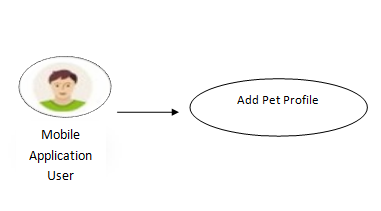
\includegraphics{32UseCase}
     \caption{Add Pet Profile}
\end{figure}
Android Application User can add pet profile details upon successful login.
\begin{table}[ht]
\centering

\label{Add Pet Profile}
\begin{tabular}{|l|l|}
\hline
Name                      & Add Pet Profile                                                                                                                                         \\ \hline
Actor                     & Android Application User                                                                                                                                \\ \hline
Brief Description         & User is able to add the pet profiles.                                                                                                                   \\ \hline
Flow of Events            & \begin{tabular}[c]{@{}l@{}}Fill the all input text fields necessary for the pet profile\\ then added profiles are saved into the database.\end{tabular} \\ \hline
Alternate Flow of  Events & If fields are missing then user can refill them.                                                                                                        \\ \hline
Pre-condition             & Some information is necessary                                                                                                                           \\ \hline
Post condition            & Added information can be viewed.                                                                                                                        \\ \hline
\end{tabular}
\caption{Add Pet Profile}
\end{table}




\newpage
\begin{figure}[H]
  \centering
    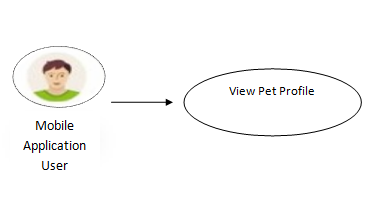
\includegraphics{33UseCase}
      \caption{View Pet Profile}
\end{figure}
Android Application User can also view the pet profile.
\begin{table}[ht]
\centering

\label{View Pet Profile}
\begin{tabular}{|l|l|}
\hline
Name                      & View Pet Profile                                                                                                       \\ \hline
Actor                     & Android Application User                                                                                               \\ \hline
Brief Description         & User is able to view the pet profile fetched from the databases.                                                       \\ \hline
Flow of Events            & \begin{tabular}[c]{@{}l@{}}After clicking the view profile button user is able to view the pet\\ profile.\end{tabular} \\ \hline
Alternate Flow of  Events & If click on any other button.                                                                                          \\ \hline
Pre-condition             & If view profile button is clicked.                                                                                     \\ \hline
Post condition            & Viewed information is fetched from database.                                                                           \\ \hline
\end{tabular}
\caption{View Pet Profile}
\end{table}





\newpage
\begin{figure}[H]  
  \centering
    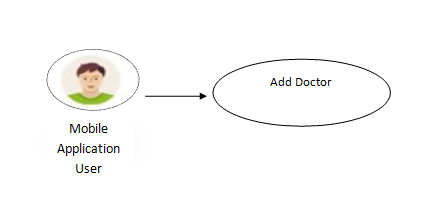
\includegraphics{45UseCase}
    \caption{Add Doctor Profile}
\end{figure}
Admin can register as a doctor if and only if the entered hospital id matches with the assigned hospital id.

\begin{table}[ht]
\centering
\label{Add Doctor Profile}
\begin{tabular}{|l|l|}
\hline
Name                      & Add Doctor                                                                                                                                           \\ \hline
Actor                     & Android Application User                                                                                                                             \\ \hline
Brief Description         & User is able to add himself as a doctor if and only if the hospital id matches.                                                                      \\ \hline
Flow of Events            & \begin{tabular}[c]{@{}l@{}}Fill the all input text fields necessary for the  profile then added profiles are\\ saved into the database.\end{tabular} \\ \hline
Alternate Flow of  Events & If fields are missing then user can refill them.                                                                                                     \\ \hline
Pre-condition             & Some information is necessary                                                                                                                        \\ \hline
Post condition            & Added information can be viewed.                                                                                                                     \\ \hline
\end{tabular}
\caption{Add Doctor Profile}
\end{table}



\newpage
\begin{figure}[H]
  \centering
    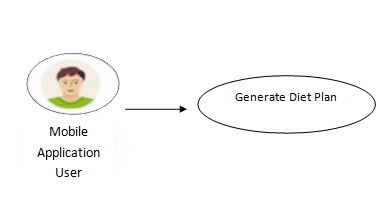
\includegraphics{34UseCase}
     \caption{Generate and Download Diet Plan}
\end{figure}
Android Application User can also generate and download the pet diet plan. Diet plans are generated on the basis of pet specie, breed(weekly or daily) ,age and type of plan.
\begin{table}[ht]
\centering

\label{Generate and Download Diet Plan}
\begin{tabular}{|l|l|}
\hline
Name                                      & View / Download Diet Plan                                                                                                                                                                             \\ \hline
Actor                                     & Android Application User                                                                                                                                                                              \\ \hline
Brief Description                         & User is able to view and download the pet diet plan.                                                                                                                                                  \\ \hline
Flow of Events                            & \begin{tabular}[c]{@{}l@{}}Select the pet specie, breed, age and type of plan (weekly or daily) then click\\ on generate plan button then diet plan will be generated from the database.\end{tabular} \\ \hline
\multirow{2}{*}{Alternate Flow of Events} & \multirow{2}{*}{If any filed is missing then no plan will be shown and downloaded.}                                                                                                                   \\
                                          &                                                                                                                                                                                                       \\ \hline
Pre-condition                             & If generate or download diet plan button is clicked.                                                                                                                                                  \\ \hline
Post condition                            & Information is fetched from database.                                                                                                                                                                 \\ \hline
\end{tabular}
\caption{Generate and Download Diet Plan}
\end{table}




\newpage
\begin{figure}[H]
  \centering
    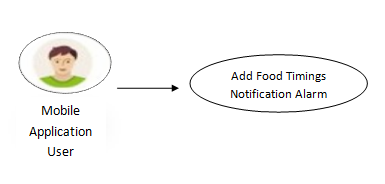
\includegraphics{36UseCase}
     \caption{Add Notificationn Alarm}
\end{figure}
Application User can add notification alarm for the multiple pets.
\begin{table}[ht]
\centering

\label{Add Notificationn Alarm}
\begin{tabular}{|l|l|}
\hline
Name                                      & Add\View Notification Alarm                                                                                                                            \\ \hline
Actor                                     & Android Application User                                                                                                                          \\ \hline
Brief Description                         & \begin{tabular}[c]{@{}l@{}}User is able to add and view the notification alarm related to\\ pet food timings for the multiple pets.\end{tabular}           \\ \hline
Flow of Events                            & \begin{tabular}[c]{@{}l@{}}Set the alarm time and then enter the pet name.\\ Then click on set alarm button. Alarm will be set down.\end{tabular} \\ \hline
\multirow{2}{*}{Alternate Flow of Events} & \multirow{2}{*}{User can delete any list item.}                                                                                                   \\
                                          &                                                                                                                                                   \\ \hline
Pre-condition                             & Pet name, time and click on set alarm button are necessary.                                                                                       \\ \hline
Post condition                            & Alarm can be deleted.                                                                                                                             \\ \hline
\end{tabular}
\caption{Add Notificationn Alarm}
\end{table}



\newpage
\begin{figure}[H]
  \centering
    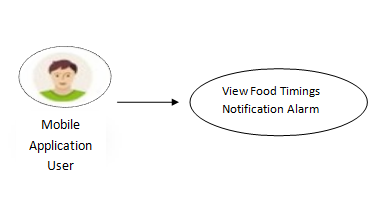
\includegraphics{37UseCase}
    \caption{View Notification List}
\end{figure}
Application User can also view the all information available on application related to notifications of pet food timings.
\begin{table}[ht]
\centering

\label{View Notification List}
\begin{tabular}{|l|l|}
\hline
Name                     & View Notification List                                                          \\ \hline
Actor                    & Android Application User                                                        \\ \hline
Brief Description        & User is able to view the notification list related to pet food timings.         \\ \hline
Flow of Events           & Click on Alarm list then user will be able to view the notification alarm list. \\ \hline
Alternate Flow of Events & User can delete any list item.User can turn off the alarm.                      \\ \hline
Pre-condition            & Click on alarm list button is necessary.                                        \\ \hline
Post condition           & Viewed information can be deleted.                                              \\ \hline
\end{tabular}
\caption{View Notification List}
\end{table}


\newpage
\begin{figure}[H] 
  \centering
    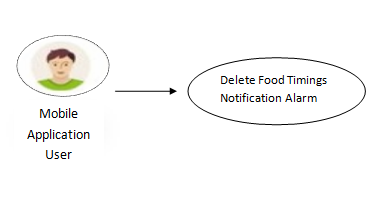
\includegraphics{38UseCase}
    \caption{Delete Notification Alarm}
\end{figure}
Application User can delete the notification list items one by one.
\begin{table}[ht]
\centering

\label{Delete Notification Alarm}
\begin{tabular}{|l|l|}
\hline
Name                     & Delete Notification Alarm                                                                                                                                         \\ \hline
Actor                    & Android Application User                                                                                                                                          \\ \hline
Brief Description        & User is able to delete the any notification list item related to pet food timings.                                                                                \\ \hline
Flow of Events           & \begin{tabular}[c]{@{}l@{}}Click on Alarm list then click on cross sign; a dialog box will be opened if yes\\ is clicked then alarm will be deleted.\end{tabular} \\ \hline
Alternate Flow of Events & User can turn off any alarm.                                                                                                                                      \\ \hline
Pre-condition            & If yes in clicked.                                                                                                                                                \\ \hline
Post condition           & Can perform on other activities or add a new alarm.                                                                                                               \\ \hline
\end{tabular}
\caption{Delete Notification Alarm}
\end{table}


\newpage
\begin{figure}[H]
  \centering
    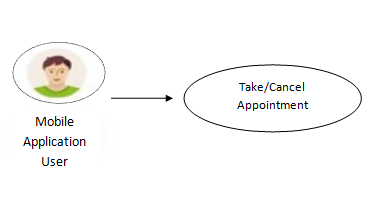
\includegraphics{46UseCase}
      \caption{Take / Cancel Appointment}
\end{figure}
Android Application user is able to take an appointment or cancel it. 
\begin{table}[ht]
\centering

\label{Take / Cancel Appointment}
\begin{tabular}{|l|l|}
\hline
Name                     & Take / Cancel  Appointment                                                                                                                                                               \\ \hline
Actor                    & Android Application User                                                                                                                                                                 \\ \hline
Brief Description        & Emails will send for the both cases if appointment is taken or cancelled.                                                                                                                \\ \hline
Flow of Events           & \begin{tabular}[c]{@{}l@{}}If appointment button is clicked then appointment email will be send.\\ If cancel button is clicked then cancel the appointment message is send.\end{tabular} \\ \hline
Alternate Flow of Events & User can view the doctors’ information.                                                                                                                                                  \\ \hline
Pre-condition            & If appoint or cancel button in clicked.                                                                                                                                                  \\ \hline
Post condition           & Can perform other activities within the application...                                                                                                                                   \\ \hline
\end{tabular}
\caption{Take / Cancel Appointment}
\end{table}


\newpage
\begin{figure}[H]
  \centering
    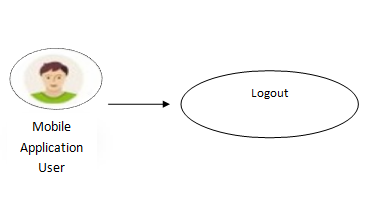
\includegraphics{41UseCase}
  \caption{Logout Details Specification}
\end{figure}

Application User is able to logout at any time.
\begin{table}[ht]
\centering

\label{Logout Details Specification}
\begin{tabular}{|l|l|}
\hline
Name                     & Logout                                                                 \\ \hline
Actor                    & Android Application User                                               \\ \hline
Brief Description        & After successful login Application User is able to logout at any time. \\ \hline
Flow of Events           & Click on logout button then user will be logout from the application.  \\ \hline
Alternate Flow of Events & Shut down the system.                                                  \\ \hline
Pre-condition            & All activates are completed no more need to stay log in.               \\ \hline
Post condition           & User is able to re login into the system at any time.                  \\ \hline
\end{tabular}
\caption{Logout Details Specification}
\end{table}

















